% !TeX root = ../thuthesis-example.tex

\chapter{系统实现}

\section{管理后台与运营数据大屏实现}



\begin{figure}[htbp]
  \centering
  
\includegraphics[width=0.9\textwidth,keepaspectratio]{figures/S10-dashboard-real.png}
  \caption{核心运营多维统计图表}
  \label{fig:S10}
\end{figure}

生鲜后台管理界面全面继承并改造了若依的管理界面。前端基于 Vue3 的 Composition API 以及 Element Plus 组件库开发，应用的主题色及图标全面更换为清新的生鲜绿色。管理后台的首页被深度定制为运营数据大屏，其整体布局采用了响应式的 Flex 网格设计，确保在不同分辨率的浏览器窗口中均能实现自适应展示。大屏顶部横向排列四个统计卡片，分别实时展示当日累计营业额、新增注册用户数、待包装处理订单数以及当前库存告警品种数量。每张卡片内嵌了独立的数字动画效果，在页面加载完成后利用 requestAnimationFrame 从零平滑递增至目标数值，营造出类似金融终端的实时刷新视觉感受。


\begin{figure}[htbp]
  \centering
  
\includegraphics[width=0.9\textwidth,keepaspectratio]{figures/S03-gateway-route-real.png}
  \caption{Gateway接口动态路由转发}
  \label{fig:S03}
\end{figure}

大屏中部嵌入了两个基于百度开源 ECharts 5.x 可视化引擎渲染的核心图表。左侧为近七日营业额趋势折线图，图表配置中将 xAxis 的 type 设置为 category 类别轴并传入日期标签，yAxis 设置为 value 数值轴且启用 splitLine 网格辅助线，series 数据类型配置为 line 折线并开启 smooth 平滑曲线渲染与 areaStyle 面积填充渐变，底色采用从深绿到透明的线性渐变，配合 animationDuration 设置为 1500 毫秒的入场动画，使折线呈现由左向右渐次绘制的流畅效果。右侧为销售品种 Top10 水平柱状图，图表将 yAxis 配置为 category 轴并按销量降序排列品种名称，xAxis 配置为 value 轴，series 数据类型为 bar 并通过 itemStyle 对每个柱条应用不同深浅的绿色渐变色，使排名靠前的品种视觉突出。两个图表实例均监听了浏览器的 resize 事件，在窗口尺寸发生变化时自动调用 chart.resize() 方法完成自适应重绘。

大屏底部展示最新五条待处理包装订单列表，每条记录包含订单编号、下单时间、购买用户昵称以及应付总金额。后端提供的接口以多表联合聚合查询方式获取上述全部数据，当日营业额的计算通过对订单表中 pay\_time 字段落在当天零点至当前时刻区间内的已付款记录执行 SUM(amount) 聚合完成。Top10 热销品种的统计则是对订单明细表按水果商品外键执行 GROUP BY 聚合后取 SUM(quantity) 累计销量降序排序并限定 LIMIT 10 条结果。待包装订单数通过对订单表执行 COUNT 函数并以状态字段等于已支付待接单条件进行过滤获得。所有聚合查询结果通过统一的 DashboardVO 视图对象封装后返回至前端。

大屏设置了每 30 秒自动刷新机制。前端组件在 onMounted 生命周期钩子中启动 setInterval 定时器，每隔 30000 毫秒重新发起数据拉取请求，获取最新的后端聚合结果后通过 Pinia 状态管理仓库更新全局数据源，各图表组件通过响应式侦听器自动感知数据变化并调用 chart.setOption() 方法完成图表重绘，保障了前台运营看板数据的敏捷更新。组件在 onUnmounted 生命周期钩子中通过 clearInterval 清除定时器，并调用 chart.dispose() 方法释放 ECharts 实例占用的内存资源，避免在页面路由切换时产生内存泄漏。

\section{水果分类、品种管理与 AOP 自动填充实现}

商品分类与品种列表是生鲜商城的基础数据。在 lgg-business 服务中，系统实现了分类与品种的完整 CRUD 模块。分类管理提供分页查询和树形层级展示，支持对分类名称、排序权重和图标的添加修改删除及条件查询。品种管理模块在分类关联的基础上支持水果名称、规格描述、单价、销售状态以及主图的维护。系统在业务层对分类名称施加了唯一性校验约束，在新增或修改分类名称时先通过持久层 Mapper 查询是否已存在同名记录，若存在则抛出自定义业务异常阻止操作。商品品种在上架前强制要求已经完成主图上传，后端在变更商品状态为在售时会检查主图 URL 是否为空，若未上传主图则拒绝上架请求并返回相应的提示信息。

水果主图在上传时，后端接收前端通过 multipart/form-data 方式提交的文件流，并调用封装好的 MinIO 工具类完成对象存储写入。MinIO 工具类的核心是在 Spring 容器中注册的 MinioClient 单例 Bean，其初始化配置通过 application.yml 中的自定义属性注入 endpoint 地址（本地部署为 http://127.0.0.1:9000）、accessKey 访问密钥和 secretKey 密钥。工具类在系统首次启动时自动检测目标存储桶 lgg-bucket 是否存在，若不存在则通过 makeBucket 方法自动创建，随后通过 setBucketPolicy 方法将桶的访问策略设置为公共只读（download），使得前端能够直接通过 HTTP URL 访问已上传的图片资源而无需附加鉴权签名。文件上传过程中，工具类首先通过 URLConnection.guessContentTypeFromName 方法探测文件的 MIME 类型，然后为文件生成基于 UUID 的唯一存储路径以避免文件名冲突，最终调用 MinioClient 的 putObject 方法将文件流写入对象存储并返回由 endpoint、桶名与文件路径拼接而成的完整静态访问 URL。在此基础上，系统进一步实施了品牌视觉升级与静态资源托管改造。生鲜的全新品牌主标、方形品牌图标以及高清青柠背景图和混合水果篮图均已被上传并持久化托管于 MinIO 对象存储中。管理后台前端与微信小程序对应的 logo.png 均已替换为全新的品牌矢量图标；同时，登录页面（login.vue）与注册页面（register.vue）的背景样式已被重构为动态引用托管在本地 MinIO 上的青柠切片背景图。这种将前后台核心静态资源完全剥离并交付分布式对象存储托管的架构设计，不仅大幅度缩减了前端打包时的静态制品体积，还打通了平台视觉资产的动态更新闭环。

为了消除在持久层频繁手动注入创建时间、修改时间和操作人的低效操作，项目设计了基于 Spring AOP 的公共字段自动填充机制。系统首先自定义了 AutoFill 注解，该注解接收一个 OperationType 枚举参数用于区分当前操作是插入还是更新。开发人员只需将该注解标记在持久层 Mapper 接口的方法声明上即可激活自动填充。AOP 切面类 AutoFillAspect 通过 Around 环绕通知拦截所有被 AutoFill 注解标记的方法调用。切面在执行目标方法前的增强逻辑如下：首先通过 JoinPoint 的 getSignature 方法获取当前被拦截方法的签名信息，将其强制转换为 MethodSignature 类型后调用 getMethod 方法获得 Method 对象。随后从 Method 对象上提取 AutoFill 注解实例并读取其 value 属性以确定当前操作类型。接下来，切面通过 JoinPoint 的 getArgs 方法获取方法的实际参数数组，取出第一个参数即为待持久化的实体对象。对于插入操作，切面通过 Java 反射机制调用实体类中预定义的 setCreateTime、setUpdateTime、setCreateUser 和 setUpdateUser 四个 setter 方法，分别注入 LocalDateTime.now() 当前时间戳与从线程上下文 BaseContext 中提取的当前登录用户 ID。对于更新操作，则仅调用 setUpdateTime 和 setUpdateUser 两个 setter 方法注入修改时间与修改人信息。BaseContext 是一个基于 ThreadLocal 的静态工具类，在若依框架的安全过滤器链中，每个经过身份认证的 HTTP 请求到达 Controller 之前，拦截器会将当前用户 ID 存入 ThreadLocal 共享变量，使得后续业务层和持久层的任意代码都可以通过 BaseContext.getCurrentId() 透明地获取当前操作人信息而无需显式传参。

\section{订单与模拟支付闭环（OpenFeign 远程状态调用）}




\begin{figure}[htbp]
  \centering
  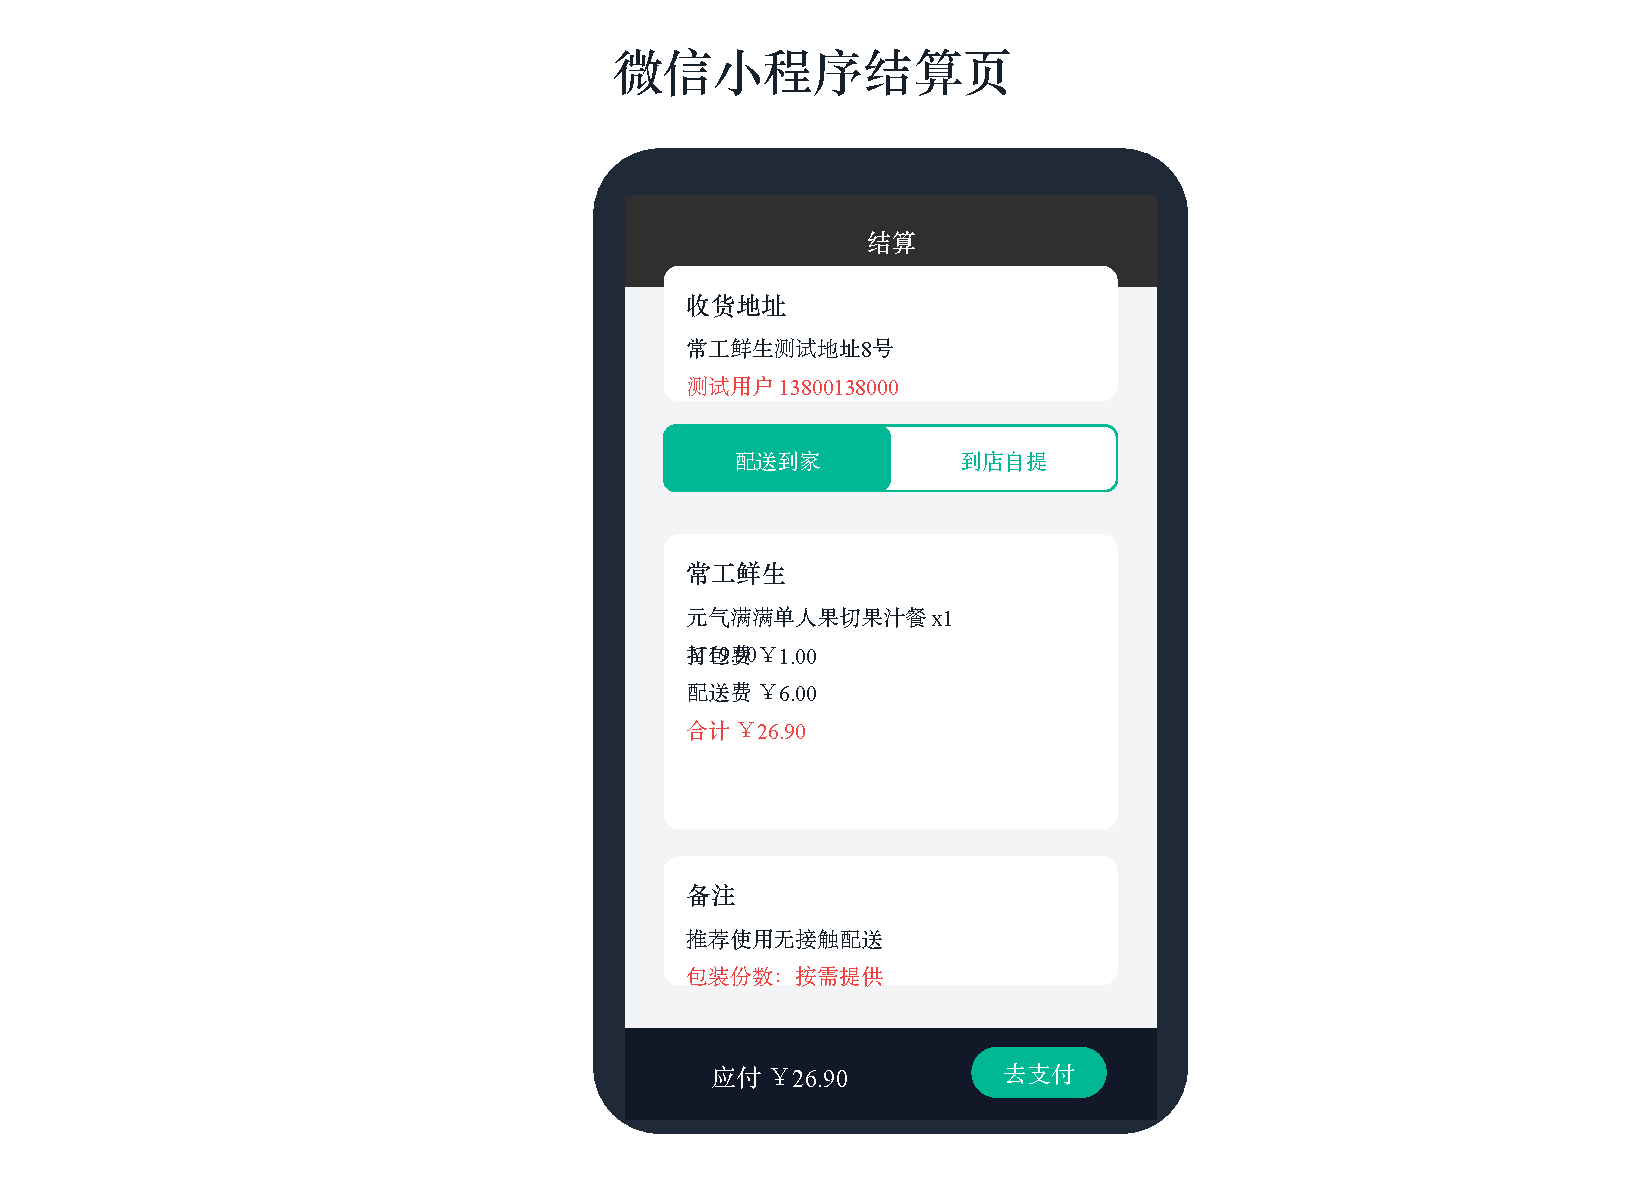
\includegraphics[height=0.40\textheight,keepaspectratio]{figures-pdf/S07-mp-checkout.pdf}
  \caption{微信小程序商品结算UI}
  \label{fig:S07}
\end{figure}

用户在小程序端结算商品并确认收货信息后提交订单，此时系统为该订单生成唯一的业务订单号并将订单状态初始化为待付款。订单的全生命周期状态机设计了六个核心状态节点，分别为待付款、已支付待接单、已接单处理中、已包装待配送、配送中以及已完成。每个状态的流转都遵循严格的单向递进规则，例如已支付状态只能由待付款状态转入且不可逆向回退，已包装状态必须由已接单状态触发且需要后台运营人员在管理界面手动确认。这种单向状态机设计确保了订单在整个生命周期中的数据一致性与业务可追溯性。当订单处于待付款状态超过 15 分钟且用户未完成支付时，系统预留了定时任务取消接口用于后续集成订单超时自动关闭功能。



\begin{table}[htbp]
  \centering
  \caption{订单生命周期状态流转表}
  \label{tab:order_status}
  \begin{tabular}{llp{0.6\textwidth}}
    \toprule
    状态值 & 状态名称 & 触发条件与流转限制 \\
    \midrule
    0 & 待付款 & 用户提交结算确认单，默认初始状态 \\
    1 & 已支付待接单 & 用户完成模拟微信扣款，由 Feign 远程调用更新 \\
    2 & 已接单处理中 & 运营人员在后台确认为有效订单并分配处理 \\
    3 & 已包装待配送 & 仓库人员完成货品打包并录入物流单号 \\
    4 & 配送中 & 快递系统回调或手动变更为发货状态 \\
    5 & 已完成 & 用户在小程序端点击确认收货或系统超时自动确认 \\
    \bottomrule
  \end{tabular}
\end{table}


\begin{figure}[htbp]
  \centering
  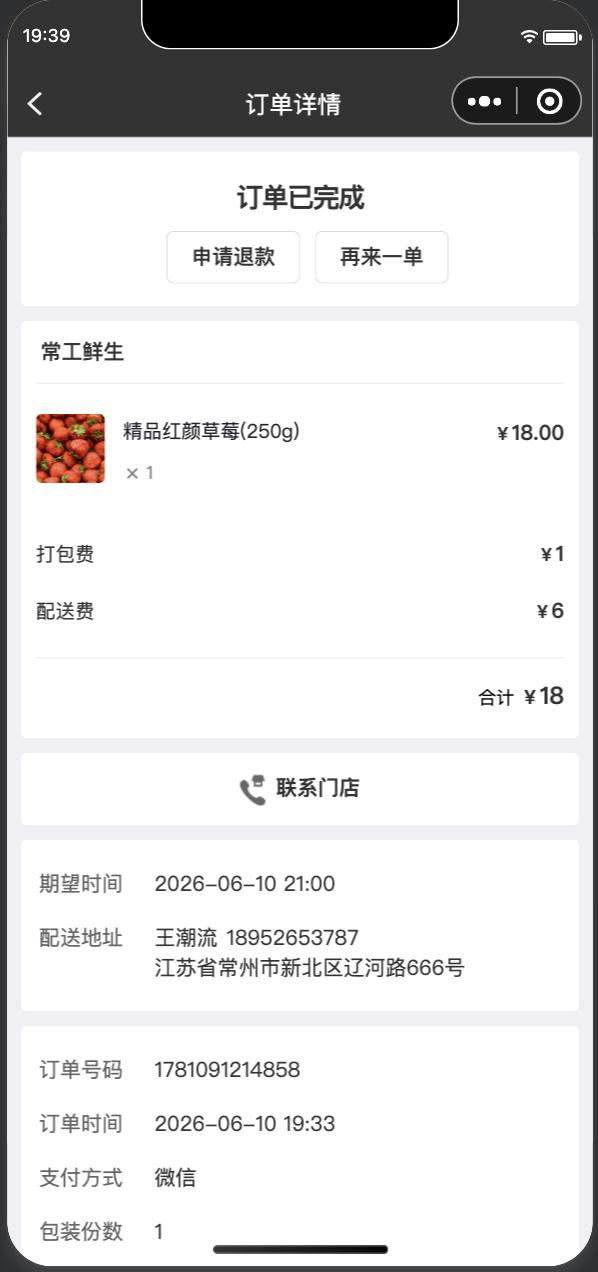
\includegraphics[height=0.40\textheight,keepaspectratio]{figures-pdf/S14-mp-order-detail.pdf}
  \caption{微信小程序订单详情UI}
  \label{fig:S14}
\end{figure}

为了保证支付系统的安全隔离与职责分离，项目专门解耦并设立了单独运行的 lgg-pay 支付微服务。该服务独立运行在 8085 端口，在 Nacos 中注册的服务名为 lgg-pay，与核心业务服务之间通过声明式的 OpenFeign 客户端进行强类型远程通信。当用户在小程序端确认支付后，前端将订单号和支付金额作为参数提交至支付服务的模拟扣款接口。支付服务在验证请求参数的合法性后执行模拟扣款逻辑，该逻辑在测试环境中省略了微信支付 SDK 的真实签名与证书校验环节，直接返回扣款成功响应。


\begin{figure}[htbp]
  \centering
  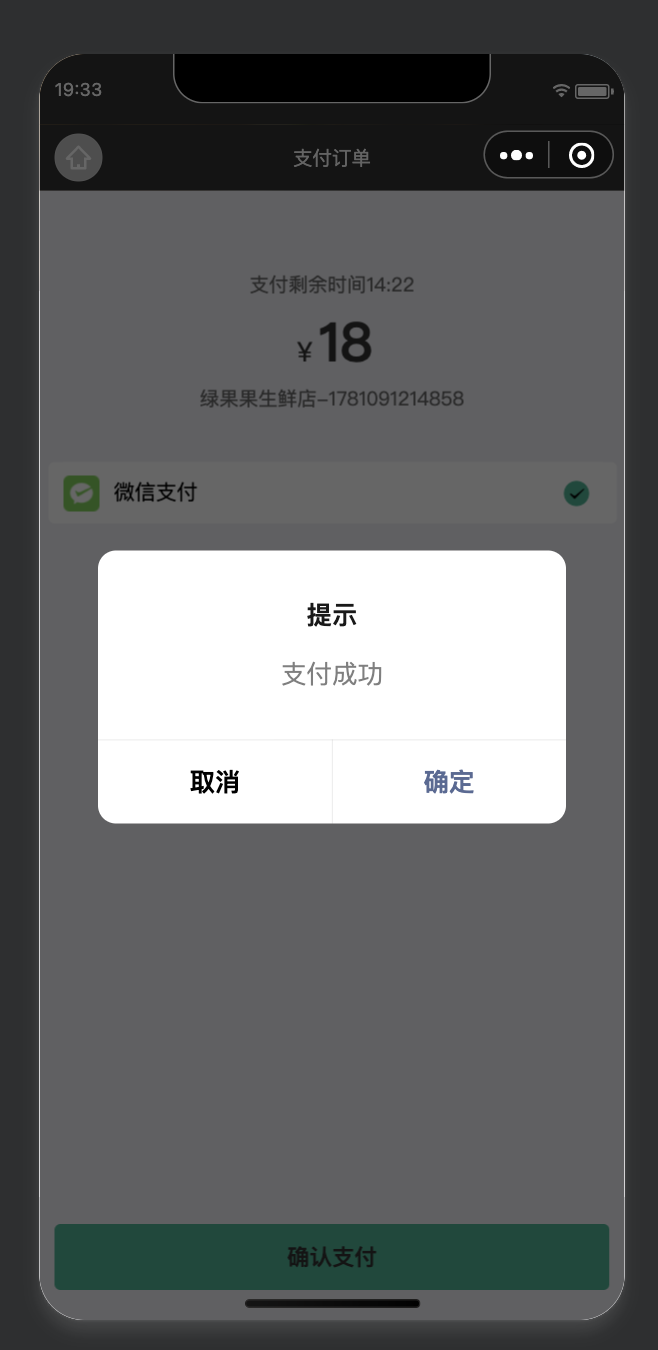
\includegraphics[height=0.40\textheight,keepaspectratio]{figures/S13-mp-pay-success.png}
  \caption{微信小程序支付成功界面}
  \label{fig:S13}
\end{figure}

在模拟支付回调阶段，系统对 OpenFeign 接口执行了异常健壮性优化。由于微信异步支付回调在到达服务端时不携带当前用户上下文信息，且业务订单号可能包含字母前缀，因此在业务服务核心接口的订单查询逻辑中，系统首先尝试通过订单号精确匹配查询。如果首次查询未能命中记录，则进入兼容查询分支。在兼容查询中，系统先通过正则表达式判断传入的订单号是否为纯数字字符串，只有当订单号完全由数字组成时才调用 Long.valueOf 将其转换为主键 ID 并执行主键查询，从而规避了对含有字母前缀的订单号强行执行类型转换导致的 NumberFormatException 运行时异常。对于非纯数字订单号，系统则直接通过业务服务持久层的多条件分页查询 pageQuery 降级查找。这一设计保证了支付回调链路在各种订单号格式下的稳定运行。

OpenFeign 客户端的调用配置中设置了 connectTimeout 连接超时为 5000 毫秒以及 readTimeout 读取超时为 10000 毫秒，防止因网络波动或目标服务响应缓慢导致调用方线程长时间阻塞。同时，为了解决异步环境下的认证问题，我们针对微服务内部的 Feign 相互调用进行了局部的安全规则放行。当模拟扣款动作执行成功，支付服务通过 OrderFeignClient 声明式接口远程调用业务服务的订单状态更新核心接口，将底层 MySQL 中对应订单记录的流转状态由待付款更改为已支付待接单，并记录实际付款完成时间戳。


\begin{figure}[htbp]
  \centering
  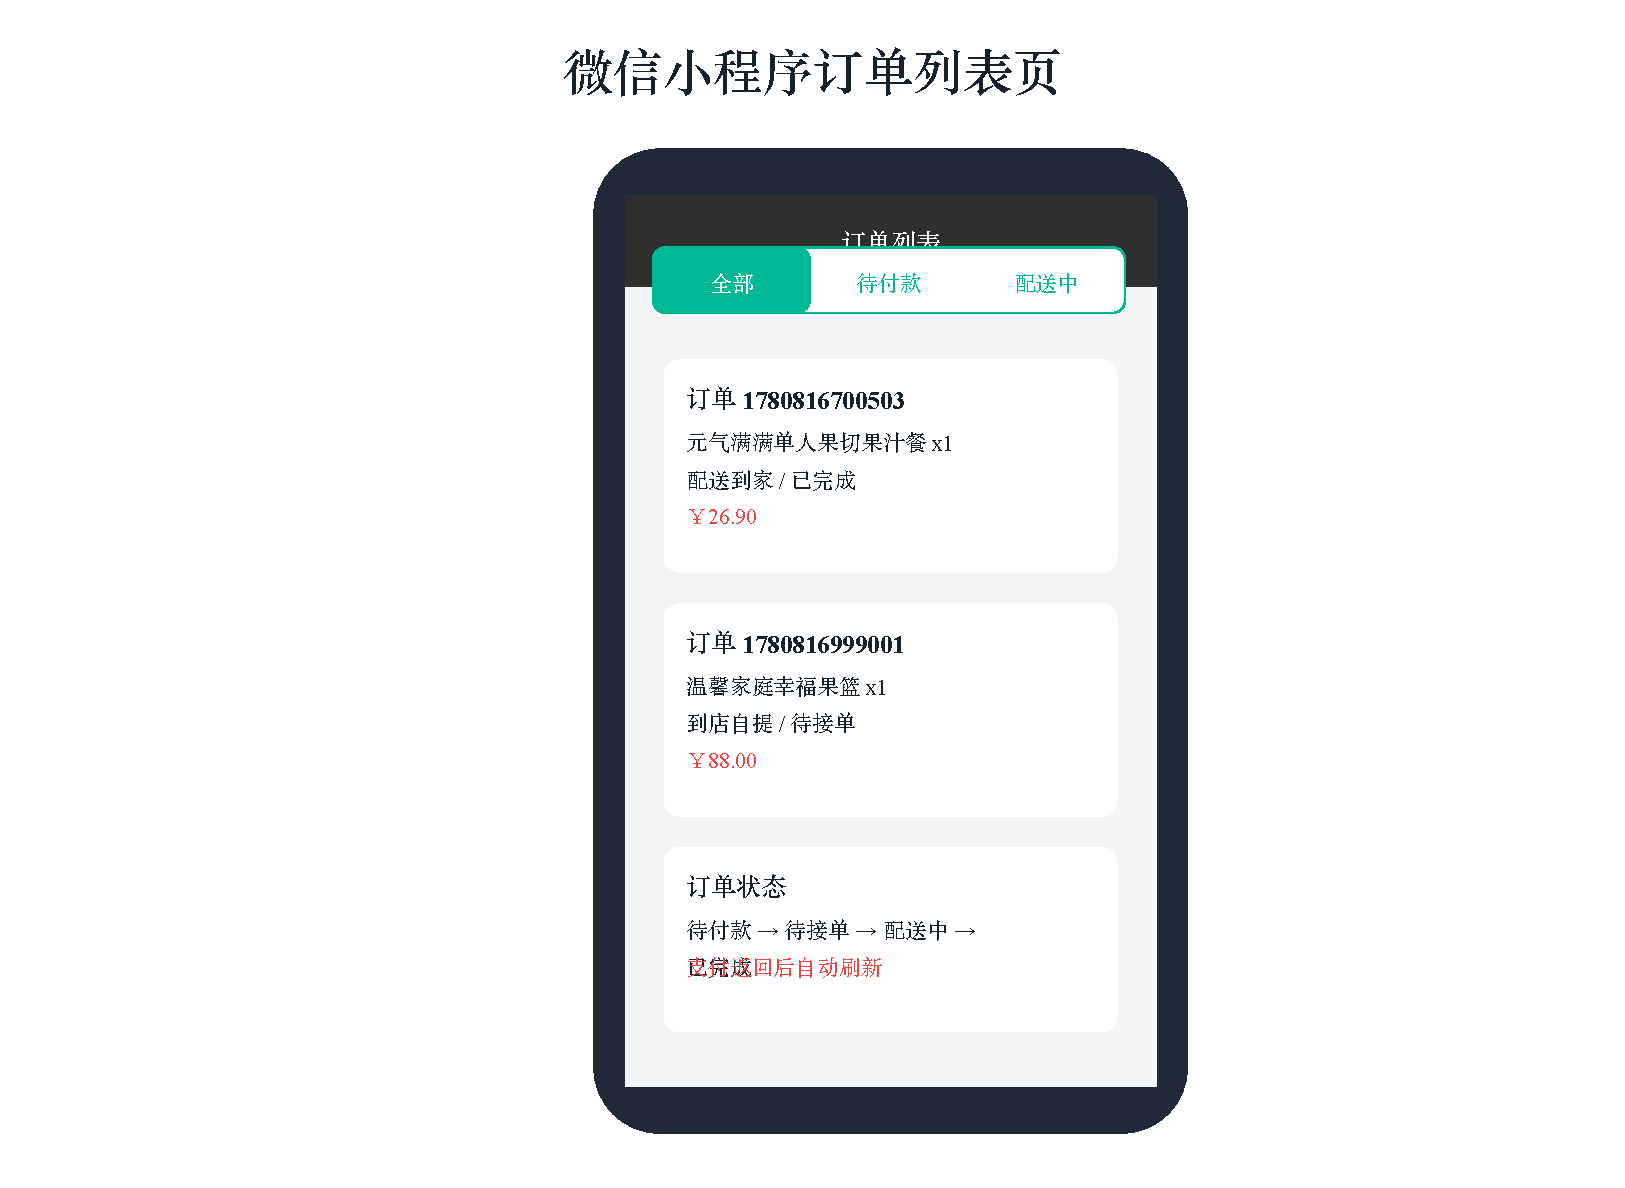
\includegraphics[height=0.40\textheight,keepaspectratio]{figures-pdf/S15-mp-order-list.pdf}
  \caption{微信小程序订单列表UI}
  \label{fig:S15}
\end{figure}


\begin{figure}[htbp]
  \centering
  
\includegraphics[width=0.9\textwidth,keepaspectratio]{figures/S04-feign-call-real.png}
  \caption{OpenFeign跨服务远程状态调用}
  \label{fig:S04}
\end{figure}

上述截图 S07 展示了微信小程序端的商品结算页面，用户可以在该页面确认购物车中选购的水果品种及数量、选择或新增收货地址、查看应付总金额并提交订单。截图 S13 展示了微信小程序支付成功界面，用户可在该页面查看支付状态、订单编号及支付金额。截图 S04 则展示了支付服务控制台的日志输出，能够清晰看到 OpenFeign 远程调用业务服务接口的完整 HTTP 请求与响应信息，包括目标服务名、请求路径、请求方法以及返回的 200 状态码。

\section{WebSocket 消息广播与 RabbitMQ 解耦实现}


为实现支付与后台通知的高鲁棒异步解耦，当支付微服务 lgg-pay 完成对业务服务的 Feign 订单状态更新并获得成功响应后，它会将付款订单的业务单号作为消息体投递至 RabbitMQ 交换机中。本系统选用 Direct Exchange 直连交换机模式，这意味着消息会根据精确匹配的 Routing Key 被路由到绑定了相同 Key 的目标队列中。支付服务通过 Spring AMQP 的 RabbitTemplate 发送消息时指定交换机名称为 pay.exchange、路由键为 pay.success，消息体为 JSON 序列化后的订单支付成功事件对象，其中包含订单号、支付金额和支付时间三个核心字段。


\begin{figure}[htbp]
  \centering
  
\includegraphics[width=0.9\textwidth,keepaspectratio]{figures/S05-rabbitmq-bindings-real.png}
  \caption{RabbitMQ消息事件队列绑定}
  \label{fig:S05}
\end{figure}

通知服务 lgg-notice 中的消费者监听类采用了 RabbitListener 注解与 QueueBinding 注解的组合声明方式来完成队列与交换机的自动绑定。QueueBinding 注解中的 value 属性声明了队列名称 pay.success.queue 并通过 durable 参数设置为持久化队列，exchange 属性声明了交换机名称 pay.exchange 并设置为持久化 Topic 类型交换机，key 属性指定路由键为 pay.success。这种声明式绑定方式的核心优势在于，当通知服务首次启动时，即使 RabbitMQ 中尚未手动创建上述队列和交换机，Spring AMQP 也会根据注解声明自动完成队列创建、交换机创建以及两者之间的路由绑定操作。这一设计彻底规避了早期版本中因 RabbitMQ 中队列不存在而导致通知服务冷启动时抛出 404 NOT\_FOUND 异常并被 PM2 反复拉起的严重故障。

当消费者监听方法成功接收并反序列化消息后，首先提取订单号字段，然后构建统一格式的 JSON 推送报文。推送报文结构包含四个核心字段：type 字段固定为 ORDER\_REMINDER 用于前端消息类型分发、orderNumber 字段携带业务订单号、message 字段为中文提示语"您有新的生鲜订单，请及时包装！"、timestamp 字段记录推送时刻的 ISO 8601 格式时间戳。构建完成后，消费者调用 WebSocket 服务层的 broadcastMessage 广播方法，该方法遍历当前所有已建立 WebSocket 长连接的会话对象并逐一发送推送报文。


\begin{figure}[htbp]
  \centering
  
\includegraphics[width=0.9\textwidth,keepaspectratio]{figures/S09-admin-notification-real.png}
  \caption{管理端WebSocket实时订单提醒}
  \label{fig:S09}
\end{figure}


\begin{figure}[htbp]
  \centering
  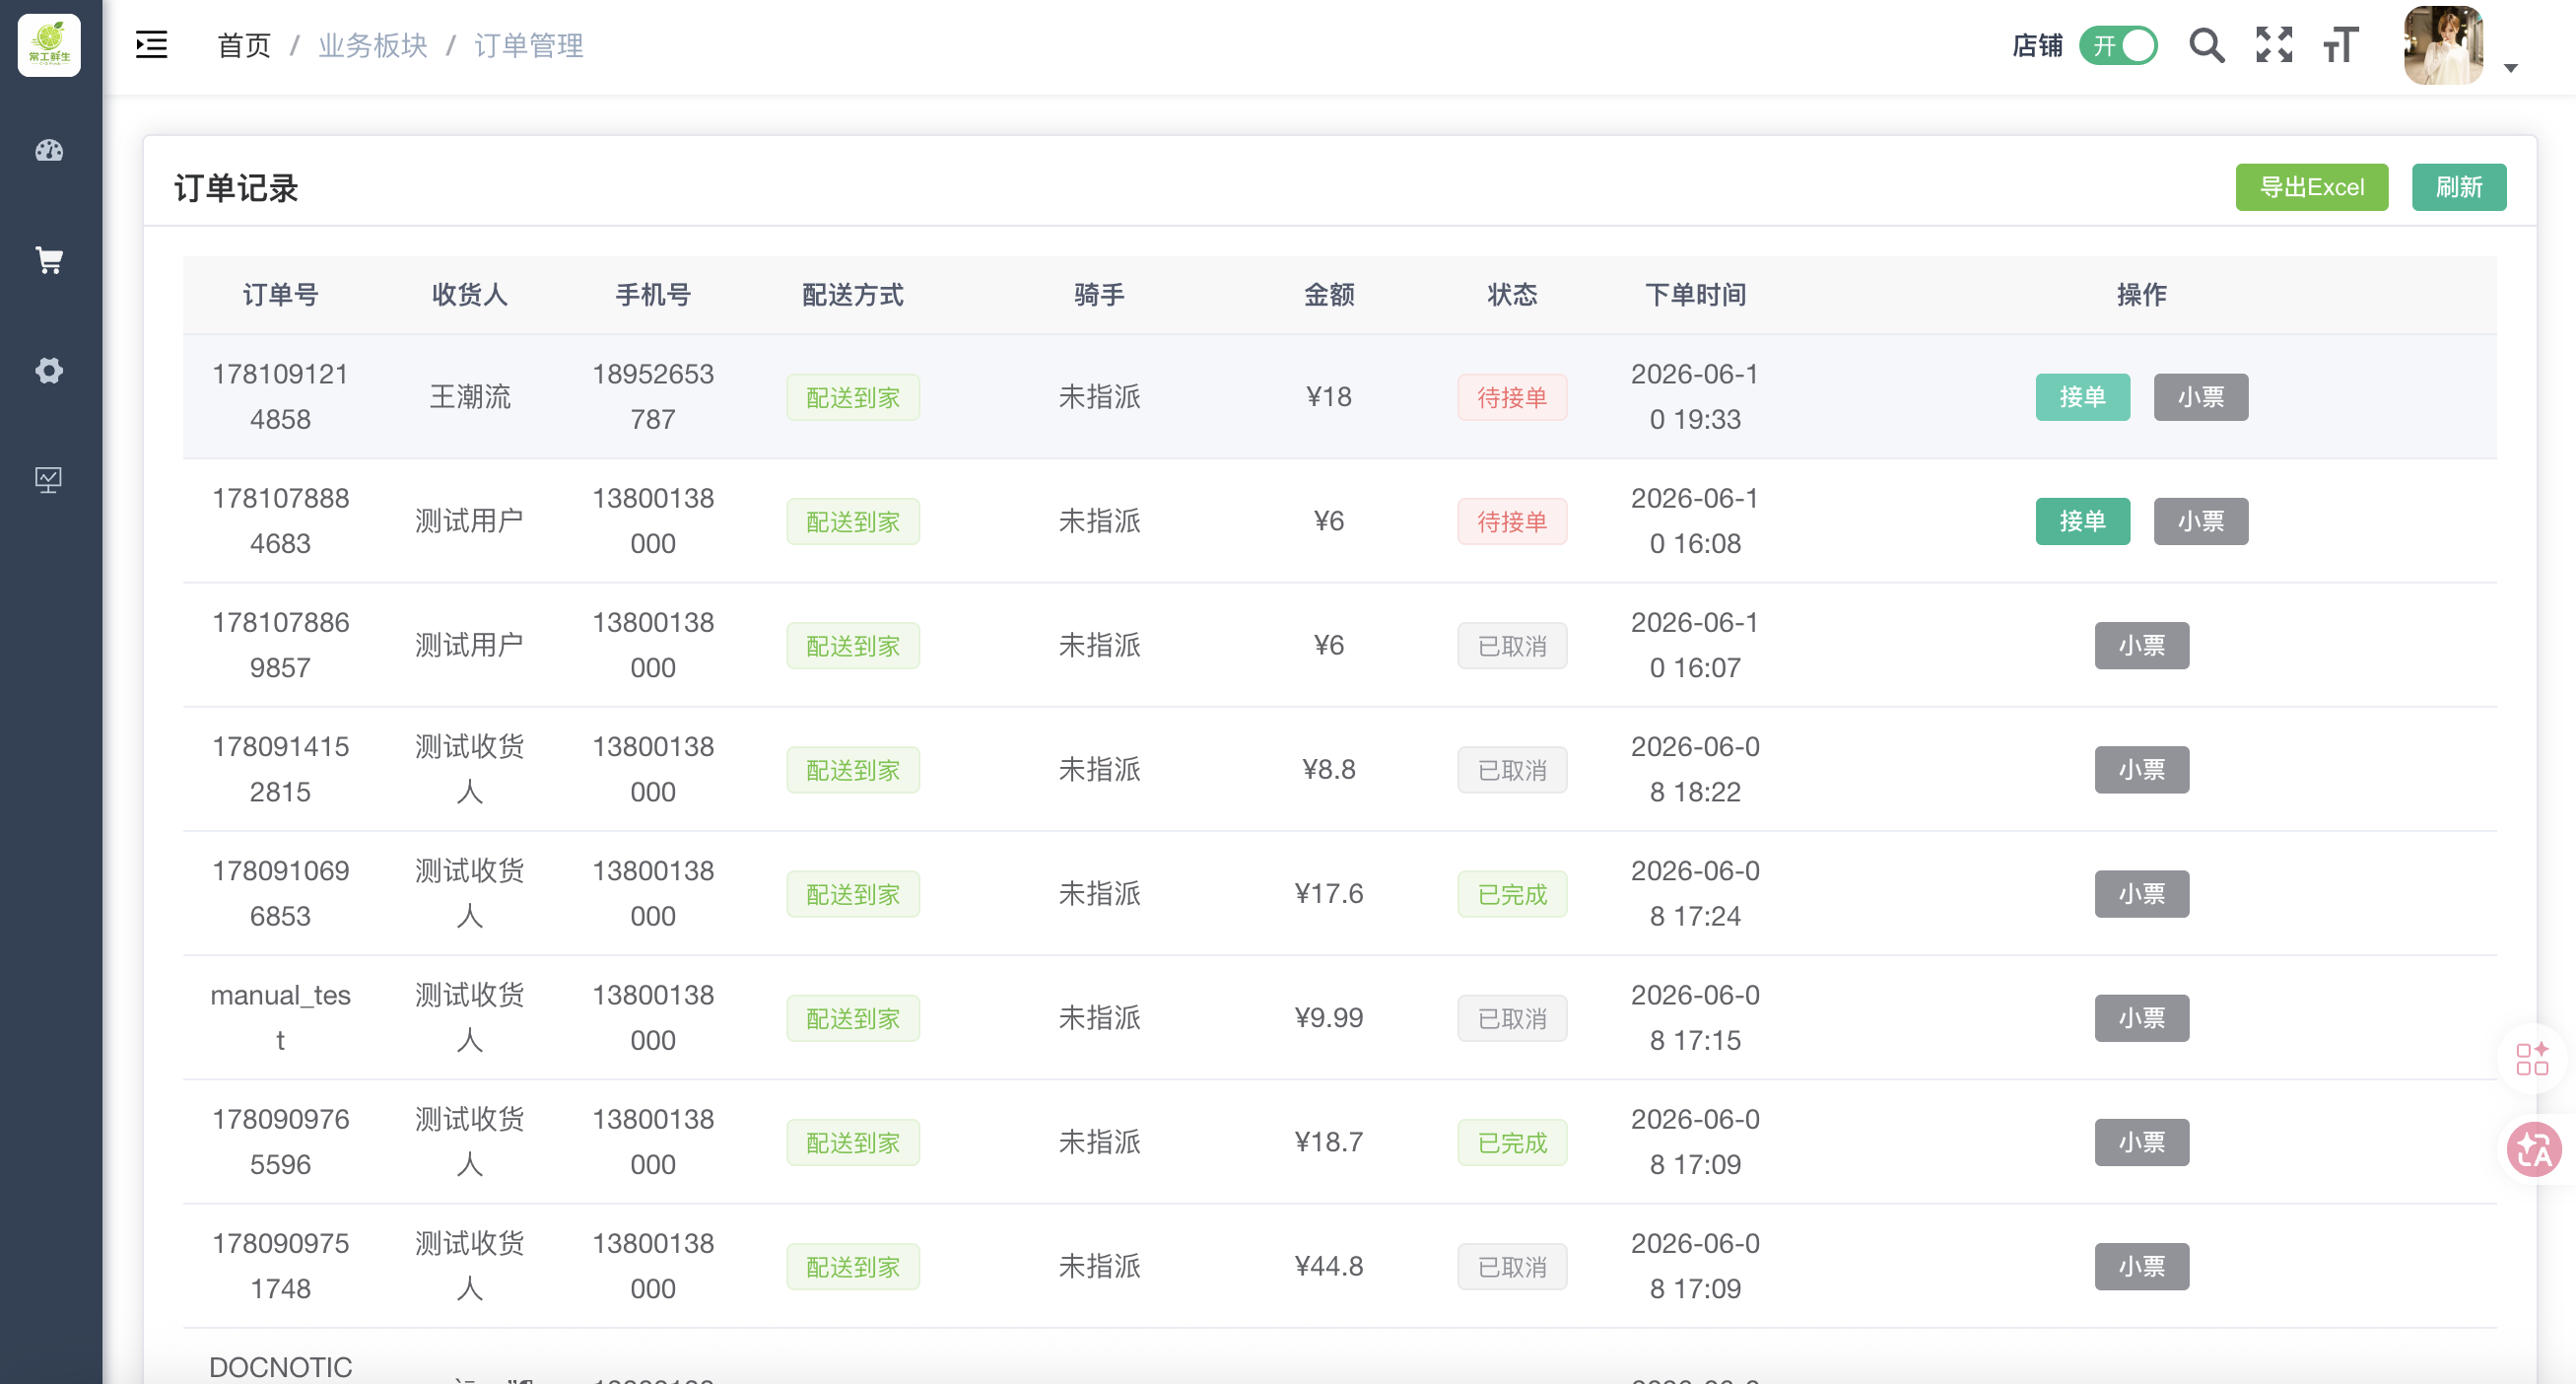
\includegraphics[width=0.9\textwidth,keepaspectratio]{figures/S16-order-status-page.png}
  \caption{订单状态实时变化页面}
  \label{fig:S16}
\end{figure}

在前端管理界面中，Vue3 组件在 onMounted 生命周期钩子中创建 WebSocket 客户端实例并连接至通知微服务的 WebSocket 端点。当前端 WebSocket 客户端收到 onmessage 事件后，首先对消息数据进行 JSON 解析，然后根据 type 字段判断消息类型。若为 ORDER\_REMINDER 类型，则立即调用 Element Plus 提供的 ElNotification 全局通知组件在页面右上角弹出订单提醒卡片，卡片标题显示"新订单提醒"、正文显示推送报文中的 message 内容以及订单号。同时，前端通过创建 Audio 对象并调用其 play 方法播放预置的提示音文件，实现听觉层面的即时提醒。ElNotification 组件的 duration 参数设置为 0 表示不自动关闭，运营人员需要手动点击关闭按钮确认已收到订单提醒，这一设计避免了高频订单场景下提醒被自动消失而遗漏的风险。

上述截图 S05 展示了 RabbitMQ 管理后台中 pay.success.queue 队列与 pay.exchange 交换机的绑定关系视图，可以看到队列已成功绑定且含有消息流转的统计数据。截图展示了管理后台在收到支付回调后，通过 WebSocket 长连接触发的实时订单提醒推送，管理端弹出的 Element Plus 全局浮动通知卡片直接验证了 WebSocket 推送链路已成功打通。截图展示了管理后台订单管理页面中订单状态的实时更新情况，当 WebSocket 推送触发后，订单列表中的状态字段随之自动刷新，无需手动刷新页面即可感知订单流转的实时变化。

\section{本地 PM2 长运行进程托管实现}

为了避免在大作业答辩现场启动大量的单独 Terminal 窗口并手动管理各项服务的生命周期，项目利用 PM2 进程管理器通过一份统一的 ecosystem.config.cjs 配置文件托管了整个微服务运行环境。该配置文件采用 CommonJS 模块格式导出一个包含 apps 数组的对象，数组中的每个元素定义了一个独立进程的完整运行参数。


\begin{figure}[htbp]
  \centering
  
\includegraphics[width=0.9\textwidth,keepaspectratio]{figures/S01-pm2-status-real.png}
  \caption{PM2服务运行状态}
  \label{fig:S01}
\end{figure}

对于各个 Java 微服务，配置项中的 name 字段设置了语义化的进程标识名称（如 lgg-admin、lgg-business、lgg-pay、lgg-notice、lgg-gateway），便于在 PM2 监控面板和日志查询中快速定位特定服务。script 字段统一指定为 java 可执行程序，args 字段则包含了 JVM 启动参数和目标 jar 包路径。JVM 启动参数中通过 -Xms128m 设置初始堆内存为 128 兆字节，-Xmx256m 设置最大堆内存为 256 兆字节，这一配置是经过反复调优后在本地开发环境中取得的最佳平衡点。将初始堆和最大堆设置为较低值可以显著减少五个 Java 进程同时运行时的总内存占用量，避免在本地 8GB 内存的开发机器上因内存不足触发操作系统 OOM Killer 强制杀死进程。同时，-Dspring.profiles.active=dev 参数显式指定激活开发环境配置文件，确保各微服务加载正确的数据源、端口和中间件连接参数。

cwd 字段为每个服务指定了工作目录，确保 jar 包中的相对路径引用能够正确解析。max\_memory\_restart 字段设置为 512M，当某个 Java 进程的实际内存使用量超过 512 兆字节时 PM2 将自动执行优雅重启，防止内存泄漏导致的渐进性性能退化。error\_file 和 out\_file 字段将标准错误输出和标准输出分别重定向至项目根目录下的 logs 子目录中的独立日志文件，便于事后排查问题时通过 pm2 log 命令或直接查看日志文件定位异常堆栈。

对于中间件进程，配置文件中同样定义了 Redis 和 Nacos 的守护配置。Redis 的 script 字段指向本地 redis-server 可执行程序并通过 args 传入默认配置文件路径。Nacos 的 script 字段指向其启动脚本 startup.sh 并附加 -m standalone 参数以单机模式启动。前端服务则配置为在固定的 8087 端口以 vite preview 预览模式运行，args 字段中包含 --port 8087 和 --strictPort 两个参数，后者强制要求 Vite 在指定端口不可用时直接报错退出而非自动漂移至下一个可用端口，从根本上消除了因端口漂移导致 Playwright 测试脚本中硬编码的 URL 失效的隐患。

通过 PM2 的统一管理，答辩现场只需执行一条 pm2 start ecosystem.config.cjs 命令即可一键拉起全部服务。运行期间可以通过 pm2 monit 命令打开实时资源监控看板，以文本仪表盘形式展示每个进程的 CPU 使用率、内存占用、运行时间和重启次数。当某个服务异常崩溃时，PM2 会在毫秒级别自动检测到进程退出事件并立即重新拉起该服务，整个恢复过程对前端用户完全透明，极大地保障了现场大作业演示的极高稳定性。
